\documentclass[]{template}

% En-tête
\renewcommand{\headrulewidth}{0.1pt}
\fancyhead[C]{} 
\fancyhead[L]{\rightmark}
\fancyhead[R]{\thepage}

% Pied de page
\newcommand{\tablemat}{~}
\renewcommand{\tablemat}{\tableofcontents}
\renewcommand{\footrulewidth}{0.1pt}
\fancyfoot[C]{} %\textbf{\thepage} 
\fancyfoot[L]{}
\fancyfoot[R]{Source coding, data compression and
channel coding}

\begin{document}

\begin{guardpage}
    \academicyear{2024-2025}
    %\guardimage{de}{0.8}
    \addtitle{ELEN0060-2: Project 2}{Source coding, data compression and
    channel coding}
    \begin{authors}{0.18}
        \addauthor{Pierre}{Lorenzen}{S203724}
        \addauthor{Abdelilah}{Khaliphi}{S204896}
    \end{authors}

\end{guardpage}

\newpage
\tablemat
\newpage

\section{Implementation}

    \subsection{Question 1}
        In the implementation for this question, we first define a node class to facilitate the creation and management of the binary tree used in the Huffman coding algorithm.\\
        
        \noindent
        Secondly, iteratively, we sort the nodes based on their probabilities at each iteration, and we merge the two lowest probabilities. This node created
        by the merge of the two lowest probabilities ones is then added to the tree with a probability equal to the sum of the two lowest probabilities. 
        The children nodes are the two nodes that were merged. The process is repeated until we have a single node left, which is the root of the tree. \\

        \noindent
        Tirdly, we generate the codes for each symbol by traversing the tree. We start at the root and assign a '0' code to the left child and a '1' code to
        the right child. We continue this process recursively until we reach a leaf node, at which point we store the generated code for that symbol.\\

        \noindent
        Finally, we reorder the symbols to be consistent with the order provided at the input of the function.\\

        \noindent
        To extend the Huffman code generation to any alphabet size $q$, we can modify the algorithm to merge the q lowest-probabilities
        nodes at each step and so build a q-ary tree, where each node has up to $q$ children.\\
        
        \noindent
        To implement this with a number of input symbols $n$ and output alphabet size of $q \geq 2$, we can
        
        \begin{enumerate}
            \item Take the $n$ symbols with their probabilities
            \item Add Dummy Symbols: If $(n-1) \; mod \; (q-1) \neq  0$, add dummy symbols of probability 0 so that:
            $(n' - 1) \; mod \; (q-1)=0$
            
            where n' is the total number of symbols (real + dummy).
            \item Maintain nodes sorted by probability.  
            \item Merge q smallest-nodes.
            \item Repeat until only one node is left.
            \item Label the edges with 0,1,\ldots,q-1.
        \end{enumerate}
        
    \subsection{Question 2}

    Initially, the dictionary is established with an empty string mapped to index 0. 
    The algorithm then iterates through each character of the input sequence, progressively building phrases.
    For each iteration, it combines the current phrase with the next character from the input to form 
    a new candidate phrase. 
    If this new phrase is not already present in the dictionary, the algorithm performs two operations:

    \begin{itemize}
        \item It appends a tuple containing the index of the current phrase (as found in the dictionary) 
            and the character that triggered the creation of the new phrase to the encoded\_sequence.
        \item It then adds the new phrase to the dictionary with a unique incremental index.
    \end{itemize}

    \noindent
    The current phrase is reset after each dictionary insertion, allowing the process to restart and 
    construct new phrases from subsequent characters. If the new phrase is already present in the dictionary,
    the algorithm continues extending it until it encounters a unique phrase.\\

    \noindent
    After processing the entire sequence, any remaining unprocessed phrase is handled explicitly 
    by adding a final tuple to the encoded sequence.\\

    \noindent
    Applying this algorithm to the given example sequence "ababcbababaaaaaaa", results in constructing 
    a dictionary that maps substrings to indices, and produces an encoded sequence consisting of tuples 
    representing dictionary indices paired with subsequent characters.\\

    \noindent
    This approach effectively exploits repeating patterns within data, significantly reducing the 
    size required for storage or transmission, making it a practical and efficient method in data 
    compression scenarios.

    \subsection{Question 3}

    As explained in the theoretical course, the Lempel-Ziv algorithms can be compared on several aspects. 
    These aspects are the dictionary construction, the parsing of the input data, 
    the encoding, the dictionary address size, the adaptivity of the algorithm, 
    the efficiency, and the on-line capability.
    See table \ref{tab:basic_vs_online} for a comparison of the two algorithms.\\
    \begin{table}[ht]
        \centering
        \setlength{\tabcolsep}{6pt}
        \begin{tabular}{|p{3cm}|p{5cm}|p{5cm}|}
            \hline
            \multicolumn{1}{|c|}{Aspect} & \multicolumn{1}{c|}{Basic Lempel-Ziv} & \multicolumn{1}{c|}{On-line Lempel-Ziv} \\ \hline
            Dictionary construction      & Grows incrementally by adding new words & Same as basic \\ \hline
            Parsing                      & Greedy: find the longest prefix in dictionary & Same as basic \\ \hline
            Encoding                     & Tuple (address of prefix, next symbol) & Same as basic but address is encoded dynamically \\ \hline
            Dictionary address size      & Fixed-size = $2^n$\newline (where n is number of bits) & Variable-length based on current dictionary size \\ \hline
            Adaptivity                   & No adaptation based on dictionary & Fewer bits used at early stages \\ \hline
            Efficiency                   & Good compression with large dictionary & More efficient in early stages due to shorter addresses \\ \hline
            On-line capability           & No & Yes, can transmit as text is read \\ \hline
        \end{tabular}
        \caption{Comparison of Basic Lempel-Ziv and On-line Lempel-Ziv}\label{tab:basic_vs_online}
    \end{table}

    \noindent
    Base on this comparison, we can conclude that the advantages of the basic Lempel-Ziv algorithm are that the compression on large dictionary is 
    more efficient than the on-line Lempel-Ziv algorithm, and that the dictionary address size is fixed. 
    The backwards of this version is that it is not adaptive, and it is not on-line.\\

    \noindent
    The advantages of the on-line Lempel-Ziv algorithm are that it is adaptive, on small and medium dictionary size the efficiency is better due to the shorter addresses, and it is on-line. The backwards of this version is that the compression
    on large dictionary is less efficient than the basic Lempel-Ziv algorithm, and that the dictionary address size is variable.\\

    \subsection{Question 4}

    To decode a LZ77 encoded text, we need first to reset the basis. The encoded text is a 
    sequence of triples (Offset, Length, NextChar). 
    To decode a full sequence of triple, the same logic is applied to each triple in the sequence.\\

    \noindent
    Firstly, \textbf{if the offset is 0 and the length is 0}, then the next
    character can be appended to the output string.\\

    \noindent
    Secondly, \textbf{if the offset is not 0 and the length is not 0}, then we 
    need to move back by the specified offset in the output string and copy 
    the specified length of characters from the output string to the output string.
    After that we can add the next character to the output string.\\

    \noindent
    This process is repeated until we have decoded the entire sequence of triples.\\

    \noindent
    \textbf{Example:}\\
    \noindent
    If the encoded text is (0, 0, 'a'),
    (0, 0, 'b'),
    (0, 0, 'r'),
    (3, 1, 'c'),
    (5, 1, 'd'),
    (7, 4, 'd'). The decoding algorithm will run like seen in the table \ref{tab:decoding}: 

    \begin{table}[ht]
        \centering
        \begin{tabular}{|c|c|c|}
        \hline
        Triple      & Current output string & Afterwards output string \\ \hline
        (0, 0, 'a') & " "                   & "a"                      \\ \hline
        (0, 0, 'b') & "a"                   & "ab"                     \\ \hline
        (0, 0, 'r') & "ab"                  & "abr"                    \\ \hline
        (3, 1, 'c') & "\color{blue}{a}\color{black}{br}"                 & "abr\color{blue}{a}\color{black}c"                  \\ \hline
        (5, 1, 'd') & "\color{blue}{a}\color{black}brac"               & "abrac\color{blue}{a}\color{black}d"                \\ \hline
        (7, 4, 'd') & "\color{blue}abra\color{black}cad"             & "abracad\color{blue}abra\color{black}d"           \\ \hline
        \end{tabular}
        \caption{Decoding of the encoded text}\label{tab:decoding}
    \end{table}

\section{Source coding and reversible (lossless) data compression}

    \subsection{Question 5}

    \noindent
    After having estimated the marginal probabilities of all the 27 symbols, determine the Huffman codes for each symbol, 
    and encoded the English text. The total length of the encoded text is $239008$ bits and 
    the compression rate is $1.9496585888338465$. 

    \subsection{Question 6}

    The average length for our Huffman code is $4.10328$ bits. \\

    \noindent
    Let's compare this value with the empirical average length.
    We can see that the empirical average length is $4.10328$. So,\\
    \[
        empirical_{avg} = 4.10328 = expected_{avg}
    \]


    \noindent
    The theoretical bounds of a Huffman code are related to how closely its average codeword 
    length approximates the entropy of the source.
    \[
        \frac{H(S)}{\log \; q} \leq \overline{n} < \frac{H(S)}{\log \; q} + 1 
    \]

    \noindent
    This means that the probabilities used to build the Huffman code match exactly the observed frequencies in the text.
    That was expected because the Huffman code is built based on the frequencies of the symbols in the text.
    This means that our algorithm works well.

    \noindent
    By knowing that the entropy in this case is \[H(S) = 4.06223\] and 
    with $q = 2$ because the size of the alphabet is 2 (the Huffman tree is a binary tree), we can calculate the bounds of the average codeword length:
    \begin{align*}
        \frac{4.06223}{\log 2} &\leq \overline{n} < \frac{4.06223}{\log 2} + 1 \\
        4.06223 &\leq \overline{n} < 5.06223
    \end{align*}
    
    \noindent
    We can see that the expected average length is $4.10328$ which is between the bounds $4.06223$ and $5.06223$.
    The value of the expected average length tells us that the Huffman code is near-optimal.

    \subsection{Question 7}

    The empirical average code length evolution with text length is shown in the figure 
    \ref{fig:evolution_avg_code_length}.\\
    
    \begin{figure}[ht]
        \centering
        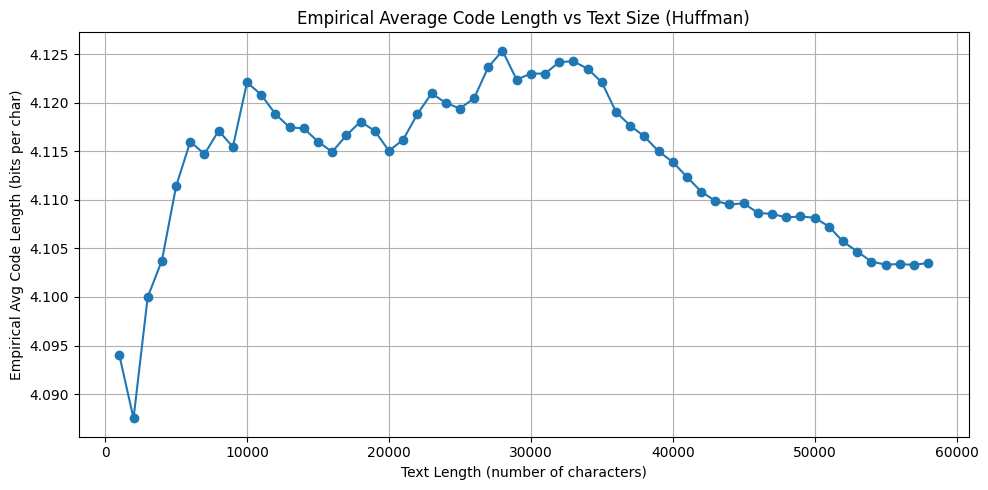
\includegraphics[width=1\textwidth]{Images/evolution_avg_code_length.png}
        \caption{Empirical average code length evolution with text length}
        \label{fig:evolution_avg_code_length}
    \end{figure}

    \noindent
    We can see that the empirical average code length is decreasing with the text length.
    This means that the Huffman code is getting better as the text length is increasing.
    We can also see that the empirical average code length is growing exponentially until we reach the 10,000 characters.
    This demonstrates that the Huffman code is not optimal for short texts.

    \subsection{Question 8}

    \subsection{Question 9}

    \subsection{Question 10}

    \subsection{Question 11}

    \subsection{Question 12}

    \subsection{Question 13}

    \subsection{Question 14}

    \subsection{Question 15}

    \subsection{Question 16}

\section{Channel coding}

    \subsection{Question 17}

    \subsection{Question 18}

    \subsection{Question 19}

    \subsection{Question 20}

    \subsection{Question 21}

    \subsection{Question 22}

\end{document}
